\section{Practical Aspects} \label{sec:practical_aspects}

We address here some issues that arise when implementing the described algorithm on a resource-constrained platform. Furthermore, we introduce many practical expedients that deal with limited sampling budget, slow control rates and finally with sim-to-real transfer.  

\subsection{Gradient Clipping} 
The policy update rule in \eqref{eq:update_rule} consists of a receding horizon \emph{mini-batch} SGD. As a consequence, the gradient variance can vary greatly between successive iterations of the algorithm. To prevent this phenomenon, which is especially evident with a small sampling budget, we clip the gradients to a user-defined threshold:
\begin{equation}
    g_i = \text{sign}(g_i) \cdot \min(|g_i|, g_{max}) 
\end{equation}
where $g_i$ is the $i$\textsuperscript{th} component of the stochastic approximation of the gradient vector and $g_{max} \in \nR{}_{>0}$ is the gradient threshold.

\subsection{Likelihood Mapping} 
The coefficient $\lambda$ in \eqref{eq:weighting} determines how ``aggressive" the weighting between different trajectories is. Adopting a constant value would give a numerically zero weight to most of the trajectories. Shifting the trajectory cost by the minimum cost as proposed in~\cite{williams_information_2017} also does not alleviate this issue. 
Especially in regions of high cost, trajectories that are locally near-optimal can be assigned very different weights. We instead propose to adopt the same technique as in~\cite{theodorou2010generalized} where $\lambda$ is scaled to better discriminate between the experienced trajectories. The modified exponential utility is then defined by,
\begin{equation} \label{eq:scale_invariant_mapping}
    \exp (-\lambda J ) = \exp \left( -h \frac{J - J_{\min}}{J_{\max} - J_{\min}} \right),
\end{equation}
which has the nice property of being invariant to the cost scale. Assume for example, that in a target reaching task, the goal pose is far away and thus the cost incurred by each sampled rollout is scaled by a common scalar factor. This factor would disappear when using the previous equation for mapping rollouts to likelihood. We show the effect of cost-scale invariance in \fig \ref{fig:exponential_mapping_comparison}. In the figure we assume that sample costs are uniformly distributed in the range between minimum and maximum cost and that the minimum cost shows a $20$\% reduction with respect to the worst rollout\footnote{This is a reasonable choice since we are in an online setup and we assume to be in a low sampling budget regime.}. We compare the exponential mapping $\mathcal{J} = \exp(-\lambda J)$ (\textit{naive}), with baseline reduction $\mathcal{J} = \exp(-\lambda (J - J_{min}))$ (\textit{baseline}) and the mapping in \eqref{eq:scale_invariant_mapping} (\textit{invariant}).

\begin{figure}[t]
    \centering
    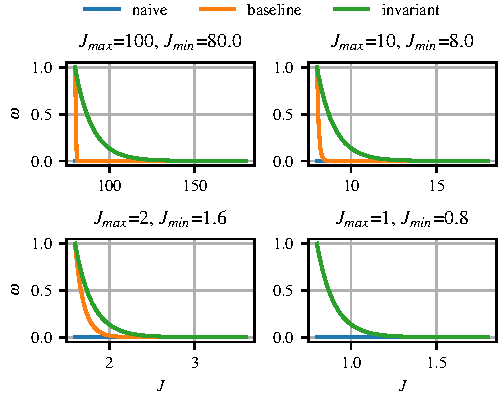
\includegraphics{figures/likelihood_mapping.pdf}
    \caption{In each plot we change the maximum and minimum cost ($80$\% of maximum cost). We set $\lambda$ and $h$ to 10 in all comparisons.}
    \label{fig:exponential_mapping_comparison}
\end{figure}

When the cost is high, the first two methods collapse all the weight to a single sample and in practice, other samples are assigned a value which is numerically zero. As a consequence, the gradient estimate in \eqref{eq:update_rule} can show a high variance. The mapping in \eqref{eq:scale_invariant_mapping} instead assigns a non-zero weight to more samples independently from the current cost scale and helps to stabilize the gradient estimate.

\subsection{Chattering}
We observed that a naive implementation of the passivity constraint leads to a chattering behavior at the constraint boundary. We start discretizing the constraint inequality to obtain a constraint that is affine in the input $\command$:
\begin{equation*}
    \int_{0}^{t + dt} \boldsymbol{\tau}_{ext}^T \command \ d\tau \approx \underbrace{\boldsymbol{\tau}_{ext}(t)^T \command(t) }_{-P_{diss}}dt + S(x_t(t)) \geq \epsilon,
\end{equation*}
which is equivalent to 
\begin{equation} \label{eq:passivity_simple}
    P_{diss} \leq \alpha E_{res},
\end{equation}
where we defined the residual energy $E_{res} = S(x_t(t))-\epsilon$. The above inequality has the drawback that when the Euler integration is performed with small time intervals, then a dangerously high power can be dissipated at any time, until very close to the lower energy limit, thus leading to chattering. It is therefore better to use a value of $\alpha < 1/dt$. Furthermore, one can easily verify that defining a passivity ZBF as $h_{pass} = S(x_t) - \epsilon$ we obtain the same formulation. The ZBF constraint reads as:
\begin{equation*}
    \dot{h}_{pass} = \dot{S}(x_t) \geq -\alpha h_{pass}
     =\alpha (\epsilon - S(x_t)).
\end{equation*}
The passivity can therefore be seen as a ZBF and consequently inherits its properties. A smaller value for $\alpha$ makes the constraint more conservative and improves its performance at the boundary. 

In order to gain a better intuitive understanding of this tuning parameter, consider the worst case scenario. In this scenario, the power flow is always equal to the maximal dissipated power allowed by the passivity constraint: $\dot{E}_{res} = - \alpha E_{res}$. Then $E_{res}(t) = E_{res}(0) e^{-\alpha t}$. A smaller $\alpha$ reduces the energy tank deplation rate  (as shown in \fig \ref{fig:worst_case_energy_profile}) at the cost of making the system more conservative.
\begin{figure}[t]
    \centering
    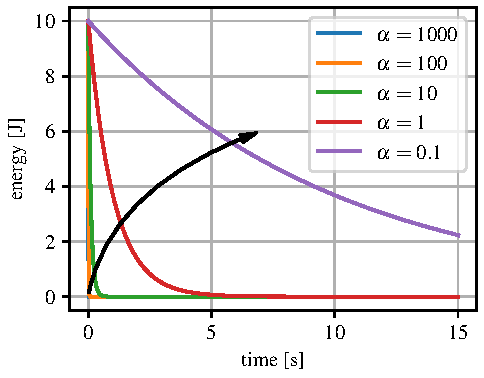
\includegraphics[width=0.8\columnwidth]{figures/worst_case_energy_profile.pdf}
    \caption{The figure shows the \textit{worst case} tank energy profile which is how the energy in the tank would evolve if the maximum allowed energy would be dissipated. The smaller the $\alpha$ the more conservative the constraint and thus the energy is depleted at a lower rate.}
    \label{fig:worst_case_energy_profile}
\end{figure}
This effect is also shown in \fig \ref{fig:tank_as_zbf} in the experiment section.

\subsection{Sampling Strategy}
At each control step, it is desirable to sample a zero input trajectory, meaning that all velocity commands are $\command_t = \bm{0}\ \forall\ t$, as this would allow the robot to stop when the goal is reached. Similarly, we would like to keep sampling the unperturbed nominal command trajectory. In fact, if we assume this to be optimal for a time instant, re-sampling would perturb it and very likely increase its associated cost. With these motivations in mind, we modify the sampling procedure such that the unperturbed and zero velocity input sequences are always in the batch of samples.

Furthermore, at the beginning of a new sampling, a subset of the best rollouts are kept and shifted back in time by the real-time number of steps elapsed since the last optimization to warm start the next iteration. 
As the sampled control is not sufficiently smooth for a practical application, we filter it using a moving window Savitzky-Golay filter~\cite{gorry1990general} before the Sequential FILTER-QP. \add{In fact, the Savitzky-Golay filter efficiently computes the optimal local polynomial approximation of the input sequence, without the need to explicitly solve an optimization problem, as it has been shown in \cite{williams_information-theoretic_2018}.} The full pipeline is visualized in \fig \ref{fig:receding_horizon}.

\begin{figure}[t]
    \centering
    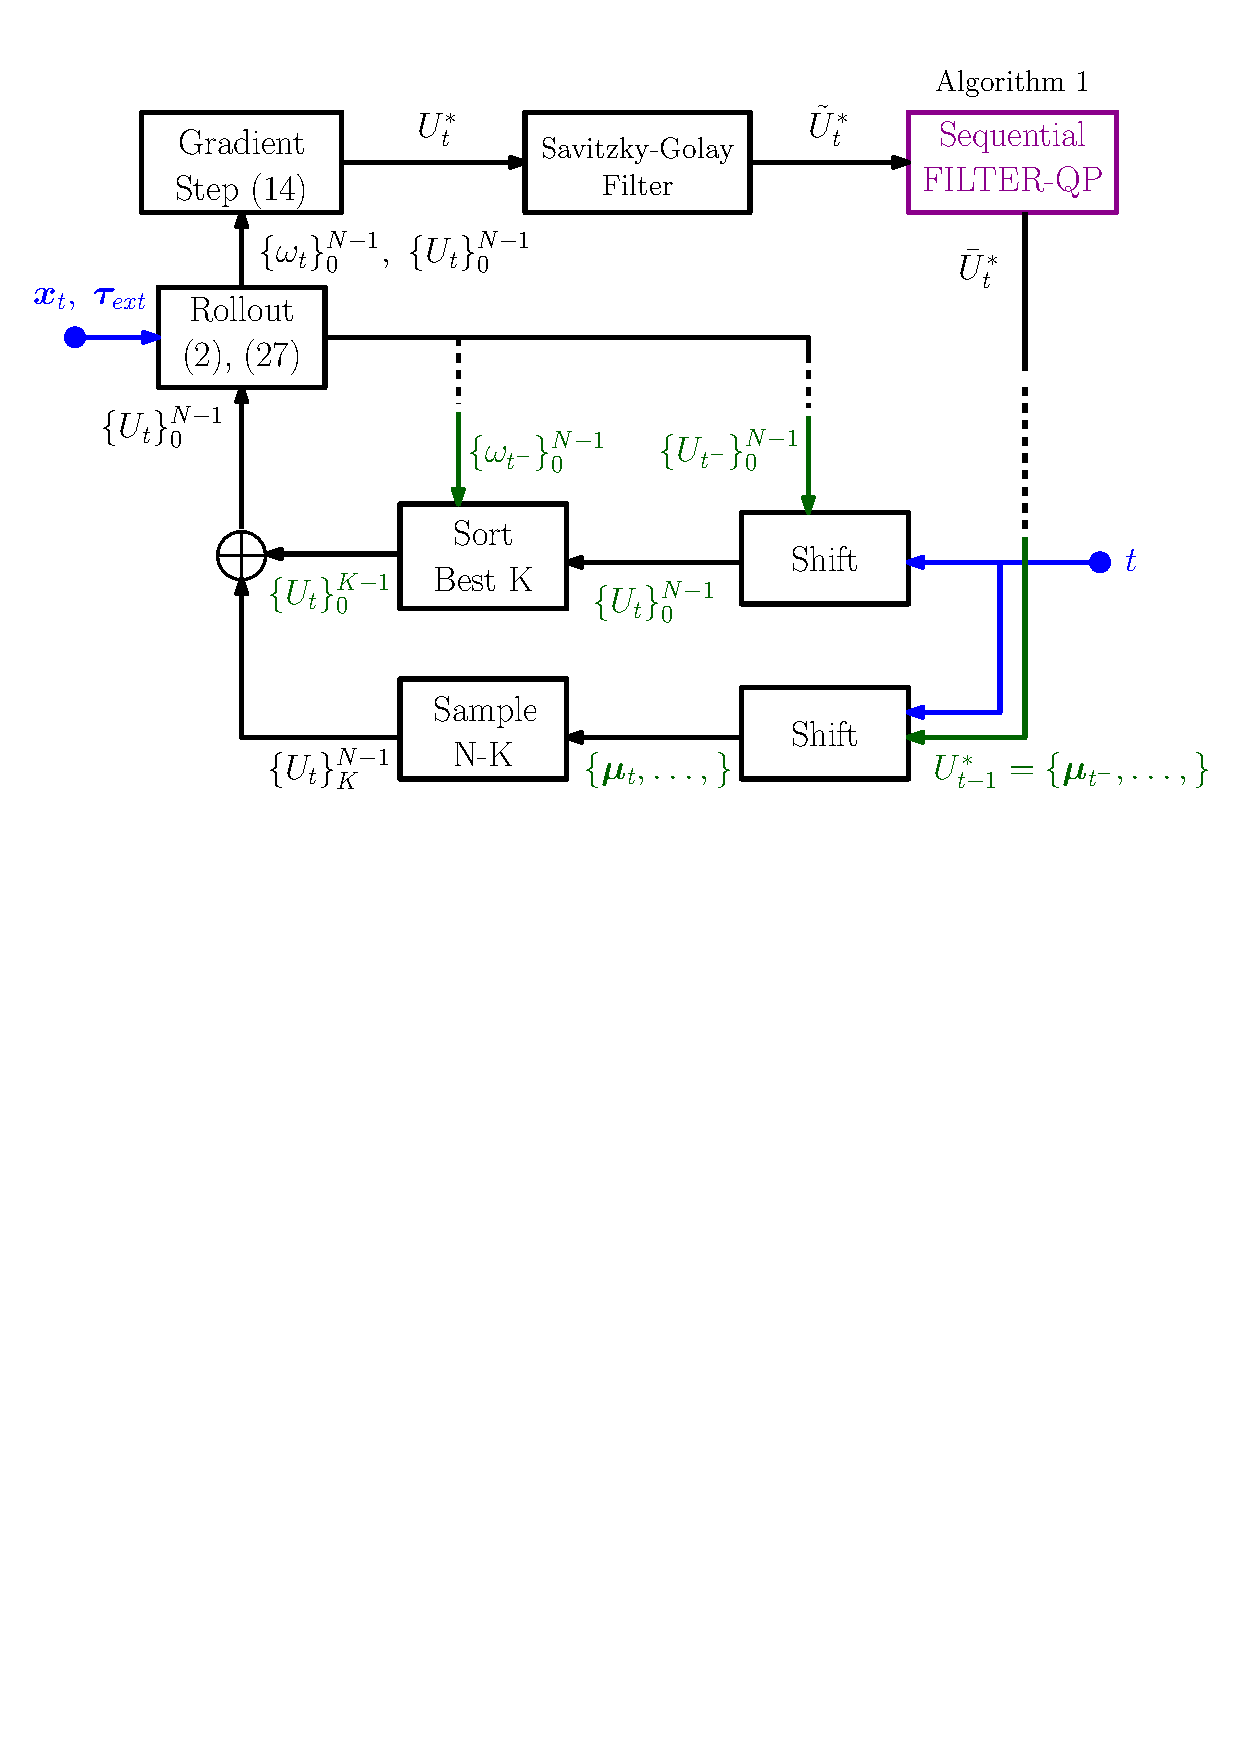
\includegraphics[width=\columnwidth]{figures/schemes/receding_horizon2.pdf}
    \vspace{0.1cm}
    \caption{The figure shows the implementation of the receding horizon scheme \add{(\emph{Reference Generation}, see \fig\ref{fig:block_scheme})}. Variables depicted in \textcolor{blue}{\textbf{blue}} and \textcolor{darkgreen}{\textbf{dark green}} represent the information available at the new optimization step and from the previous iteration, respectively. All the previous samples and the nominal trajectory are shifted by $ t - t^-$. The $K$ best input sequences (according to their weights) are reused and concatenated to a batch of $N-K$ fresh samples to perform new rollouts. The Sequential-QP block, highlighted in \textcolor{purple}{\textbf{purple}}, is optional and deployed by methods \ctrlOuter and $\Pi_{IO}$.}
    \label{fig:receding_horizon}
\end{figure}

\subsection{Contact-mesh Simplification}
A large proportion of simulation time is spent on collision detection. We reduce the component meshes to the relevant ones and simplify to primitive shapes, as shown in \fig\ref{fig:1}. We are especially interested in the collision objects belonging to the robot end-effector and the object. This adaptation tremendously reduces computation especially during the contact phase. \add{The original finger design and vendor mesh is shown in \fig\ref{fig:original_mesh}. Often, as well as in this case, the vendor mesh is a convex hull of the actual finger geometry. In our evaluation we have replaced the convex hull with the real mesh, building it with a set of 9 box primitives as shown in \fig\ref{fig:two_fingers}. Finally, to further reduce simulation time, we redesigned the hand with a single finger hook setup for non-prehensile manipulation, further reducing the needed box primitives to 3.} We observed that using the original mesh shown in \fig\ref{fig:original_mesh} results in a mean simulation rate of 0.98kHz. In contrast, the two finger mesh and hook finger mesh in \fig\ref{fig:two_fingers}-\ref{fig:hook_finger} allow mean simulation rates of 2.13kHz and 2.94kHz, respectively.

\begin{figure}[t]
\centering
\begin{subfigure}{0.3\columnwidth}
    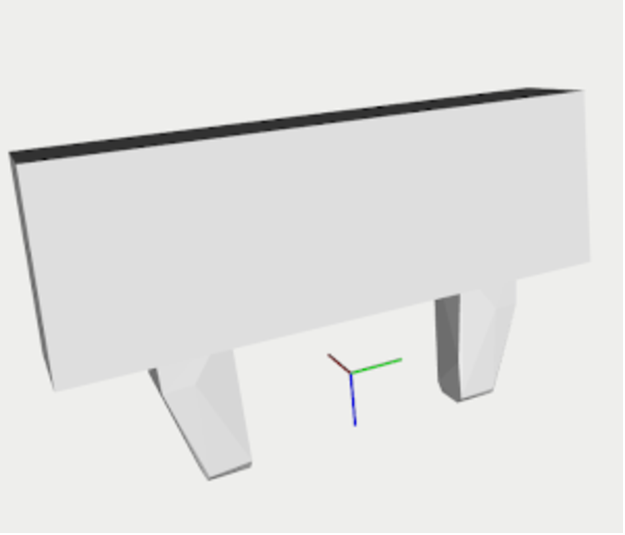
\includegraphics[width=\linewidth]{figures/hardware/mesh_cropped.pdf}
    \caption{Original mesh}\label{fig:original_mesh}
\end{subfigure}%
\hfill
\begin{subfigure}{0.3\columnwidth}
    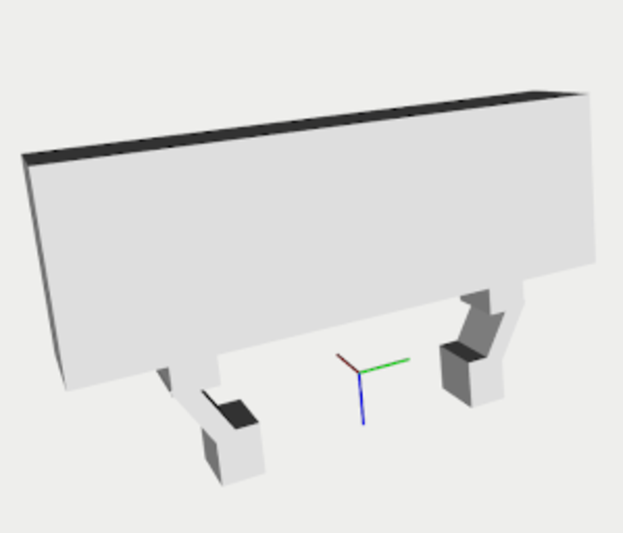
\includegraphics[width=\linewidth]{figures/hardware/doulbe_simple_cropped.pdf}
    \caption{Two fingers}\label{fig:two_fingers}
\end{subfigure}%
\hfill
\begin{subfigure}{0.3\columnwidth}
    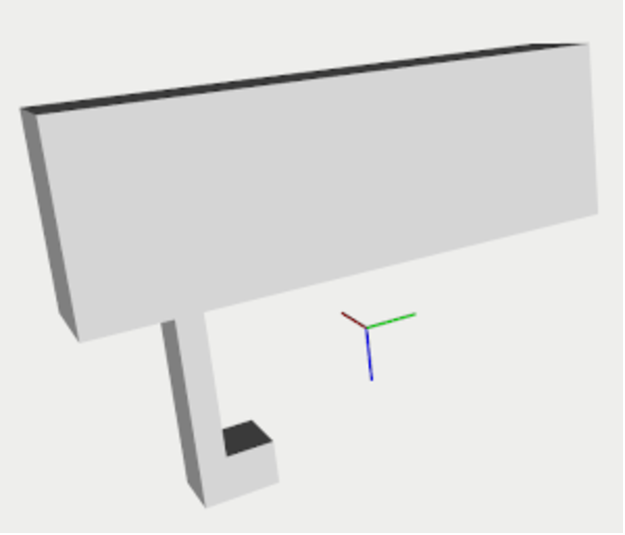
\includegraphics[width=\linewidth]{figures/hardware/single_hook_cropped.pdf}
    \caption{Hook finger}\label{fig:hook_finger}
\end{subfigure}

\caption{Original collision meshes (a) provided by the robot manufacturer are often approximated by convex hulls, which are inaccurate while also more complex representations. \add{The mesh in (b) is an exact collision shape for the original gripper made of simple box primitives. We reduce the end-effector complexity by designing a simple single-finger gripper (c) made of only 2 boxes obtaining}\remove{In contrast, a simplified mesh (shown in (b) and (c)) can bring more accuracy as well as} a computational performance gain in terms of simulation rate.\label{fig:1}}

\end{figure}

\subsection{Simulator Tuning}
\subsubsection{\add{Contact-Mesh Simplification}}
Crucial to the overall performance is the accuracy of the simulation environment (implementing \eqref{eq:eom}). Unfortunately the discrepancy between the simulator and the real physical model known as the \emph{sim-to-real} gap is unavoidable. A typical failure case consists of an over-estimation of an object's friction. In such cases, we have often observed a ``scratching" emergent behavior where the robot would rely on friction to move the object. In practice friction is hard to measure and depends on the contact patch between surfaces. On the other hand, kinematic constraints between contact points depends on the system geometry which can be accurately measured (e.g. from CAD models). Therefore solutions that exploit the latter are more likely to succeed on the real platform. One can bias the controller towards these solutions by setting, for example, a very low friction coefficient between contact bodies.

\subsubsection{\add{Simulator Stability}}

\add{A big bottleneck of the proposed approach is the computation required to forward simulate multiple samples of the system dynamics in the physics engine. The time complexity is linear in the number of rollouts, the time steps, and horizon. In order to keep a sufficiently long horizon (1s) and a good amount of samples, we increase the time discretization for forward integrating the simulated dynamics. However, simulators suffer instability issues when the time steps are large \cite{erez2015simulation}. A direct implementation of \eqref{eq:low-level-control} in the physics engine would often cause instability during the 1 second time horizon. Fortunately, the efficient simulator provides an internal PD controller \cite{raisim_pd} that allows it to track joint position and velocities with big time steps (0.015 seconds in this work) without suffering instability. The control law is then a simple P velocity controller with compensation of Coriolis and gravity terms:}
\begin{equation} \label{eq:cmd_sim}
    \vect{\tau}_{cmd} = \coriolis \dconfigRobot + \vect{g}(\configRobot) - \matr{K}_{D} \dconfigRobotError,
\end{equation}
\add{with an appropriate choice of the positive-definite diagonal gain matrix $\matr{K}_{D} \in \nR{\robotDoF\times\robotDoF}$.}

\add{Using a different low-level controller to simulate interaction trajectories inevitably introduces a model mismatch. We argue that if the real and simulated robot can track the joint velocities well, namely they have similar closed loop velocity dynamics, then we can abstract away the low-level control layer and look at the two as robots that can be directly commanded in joint velocity.}

\add{Furthermore, even when the two low-level control laws would be identical, a mismatch is still potentially possible because of numerical and model errors \cite{erez2015simulation}. Addressing these errors requires a comparative study of many simulators and involves system identification, generally a harder problem than simulation, and is outside the scope of our work. Qualitatively, our approach is a good compromise between theoretical guarantees (deploying \eqref{eq:low-level-control} on the real robot), feasibility and simulation stability (deploying \eqref{eq:cmd_sim}) on the simulated robot.}

